\chapter{Chained deep learning for image
segmentation}\label{ch:chained_deep_learning_seg}

\section{Introduction}

As mentioned in Chapter \ref{ch:introduction}, U-shaped \glspl{CNN} have been
proven a good solution for segmentation tasks in medical images, due to their
ability to capture both global and local information with relatively low
datasets.

\begin{figure}[h]
  \centering
  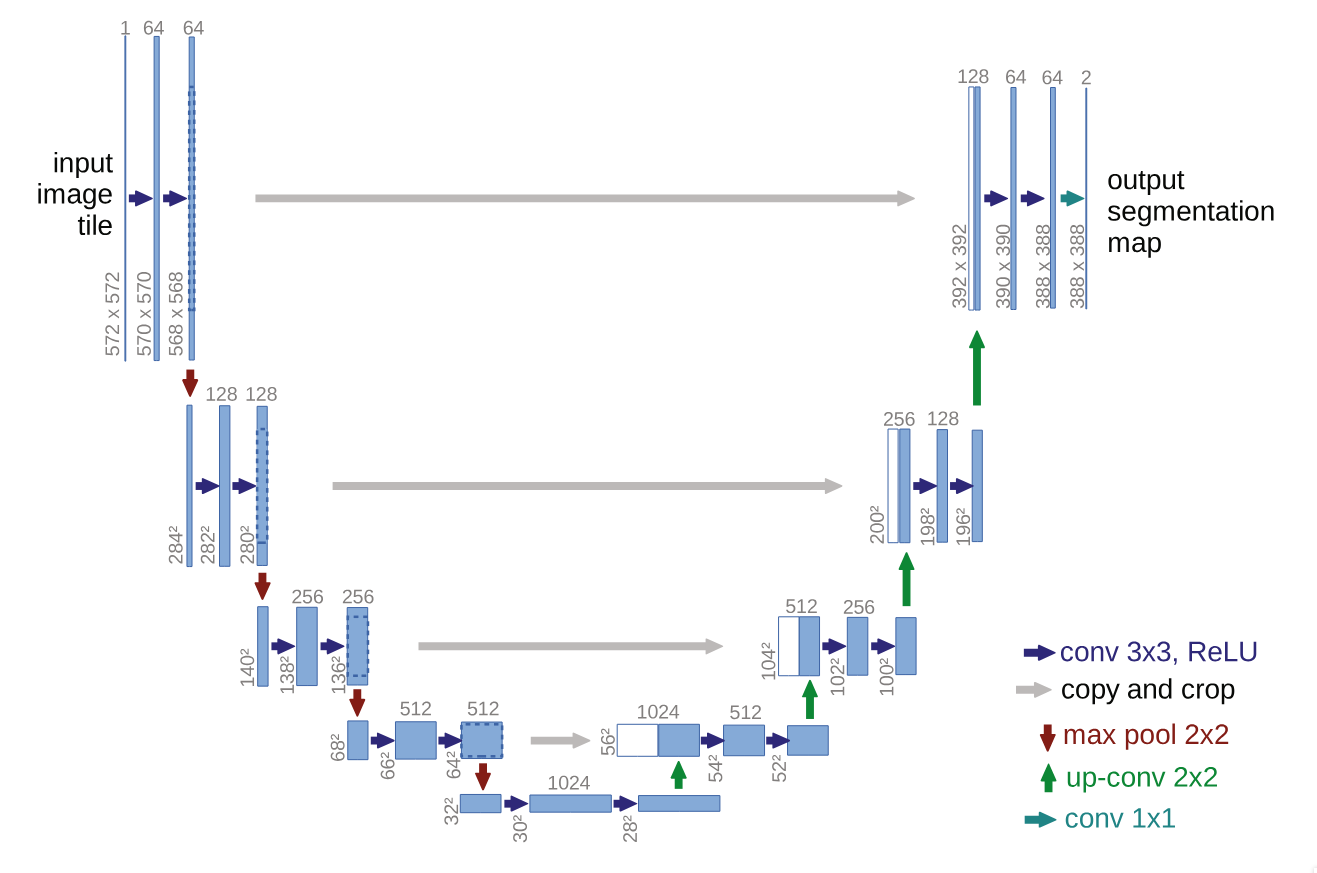
\includegraphics[width=0.8\textwidth]{Cap5/Figures/unet_architecture.png}
  \caption{Original U-NET architecture.}
  \label{fig:unet_architecture}
\end{figure}

\section{Using U-NET as a building block}

Our proposed model architecture combines the strengths of UNET with a
ResNet-34 backbone, specifically designed to work with the
TGCE$_{SS}$ loss function. The architecture is illustrated in Figure
\ref{fig:model_architecture}.

\begin{figure}[h]
  \centering
  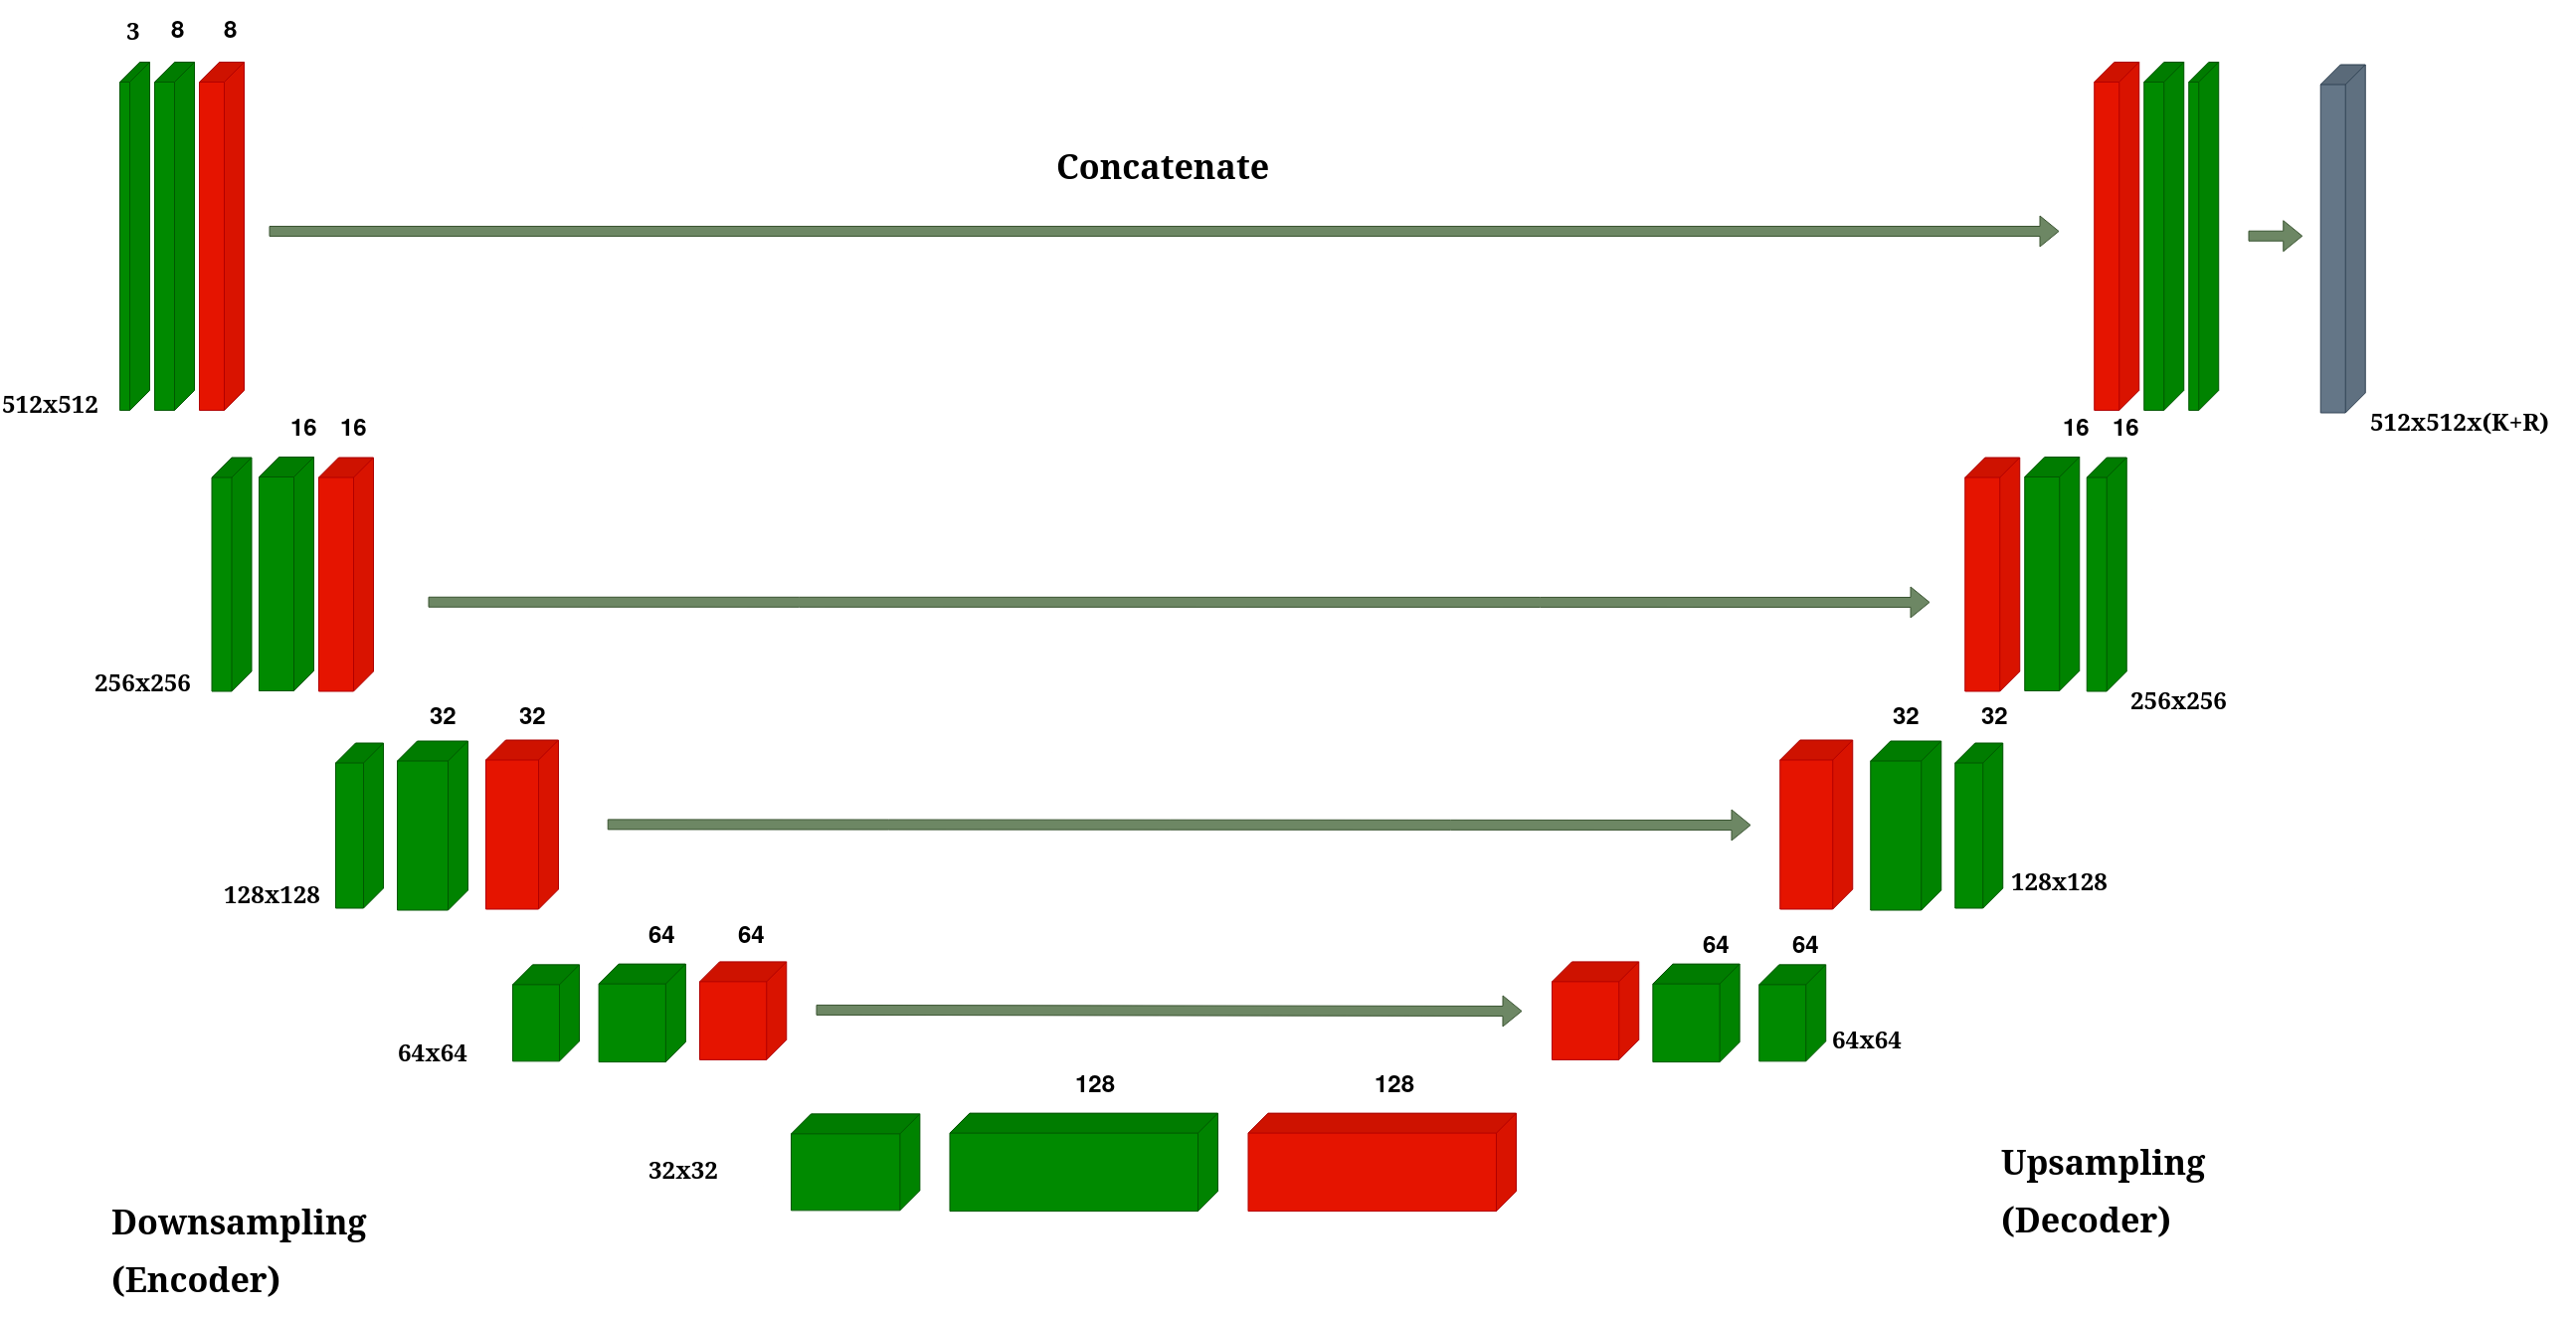
\includegraphics[width=0.8\textwidth]{Cap5/Figures/cnn_arch_overview.png}
  \caption{Overview of the proposed model architecture.}
  \label{fig:model_architecture}
\end{figure}

\subsection{Backbone Architecture}

The model employs a pre-trained ResNet-34 as its encoder backbone,
leveraging its deep residual learning framework for efficient feature
extraction. The choice of ResNet-34 provides several key advantages:
efficient feature extraction through residual connections,
pre-trained weights that capture rich visual representations, and
stable gradient flow during training. We modify the ResNet-34
backbone to serve as the encoder in our UNET architecture by removing
the final fully connected layer and utilizing the feature maps from
different stages of the network for skip connections.

\subsection{UNET Architecture}

The UNET architecture follows a traditional encoder-decoder structure
with skip connections, where the encoder path implements the
ResNet-34 structure. The decoder path employs transposed convolutions
for upsampling, creating a symmetrical architecture that effectively
captures both high-level and low-level features. The architecture
incorporates four downsampling stages in the encoder, corresponding
to the ResNet-34 blocks, and four upsampling stages in the decoder.
These stages are connected through skip connections that bridge
corresponding encoder and decoder stages, allowing the network to
preserve fine-grained details. Each convolution operation is followed
by batch normalization and ReLU activation to ensure stable training
and effective feature learning.

\subsection{Reliability Map Branch}

A key innovation in our architecture is the parallel branch dedicated
to estimating reliability maps. This branch processes the same
encoder features as the main segmentation path but focuses on
learning the confidence of each annotator. Through a series of $1
\times 1$ convolutions, the branch reduces channel dimensions while
maintaining spatial information. The final output consists of $R$
reliability maps $\Lambda_r$, one for each annotator, with values
constrained to the $[0,1]$ range through a sigmoid activation
function. This design allows the network to learn and adapt to the
varying reliability of different annotators across different regions
of the image.

\subsection{Integration with TGCE$_{SS}$ Loss}

The model produces two distinct outputs: segmentation masks
$\mathbf{\hat{Y}} = f(\mathbf{X};\theta)$ and reliability maps
$\{\Lambda_r(\mathbf{X};\theta)\}_{r=1}^R$. These outputs work in
tandem with the TGCE$_{SS}$ loss function described in Section
\ref{sec:proposed_loss}. The loss function simultaneously guides the
learning of both the segmentation masks and reliability maps,
ensuring that the model learns to balance the contributions of
different annotators based on their estimated reliability.

\subsection{Training Process}

The training process begins with the initialization of the ResNet-34
backbone using pre-trained weights, providing a strong foundation for
feature extraction. The entire network is then trained end-to-end
using the Adam optimizer with a learning rate of $10^{-4}$. The
TGCE$_{SS}$ loss function plays a crucial role in updating both the
segmentation and reliability branches, ensuring that the model learns
to effectively handle multiple annotators' inputs while accounting
for their varying reliability.
\begin{figure}[h]
  \centering
  \begin{tikzpicture}[
      node distance=1.2cm and 1.5cm,
      every node/.style={font=\footnotesize},
      box/.style={draw, rectangle, minimum width=2.5cm, minimum
      height=1cm, align=center},
      arrow/.style={-{Latex}, thick},
      roundedbox/.style={draw, rectangle, rounded corners=5pt,
      minimum width=4.2cm, minimum height=1.2cm, align=center}
    ]

    % Dataset notation
    \node[align=left] (dataset) at (-4.5,1.5) {
      \textbf{Train Dataset} \\
      $\left\{(x_n, \tilde{y}^r_n)\right\}_{r \in R_n}^{n \in \mathbb{N}}$
    };

    % Image box
    \node[box, right=2cm of dataset] (image) {%
      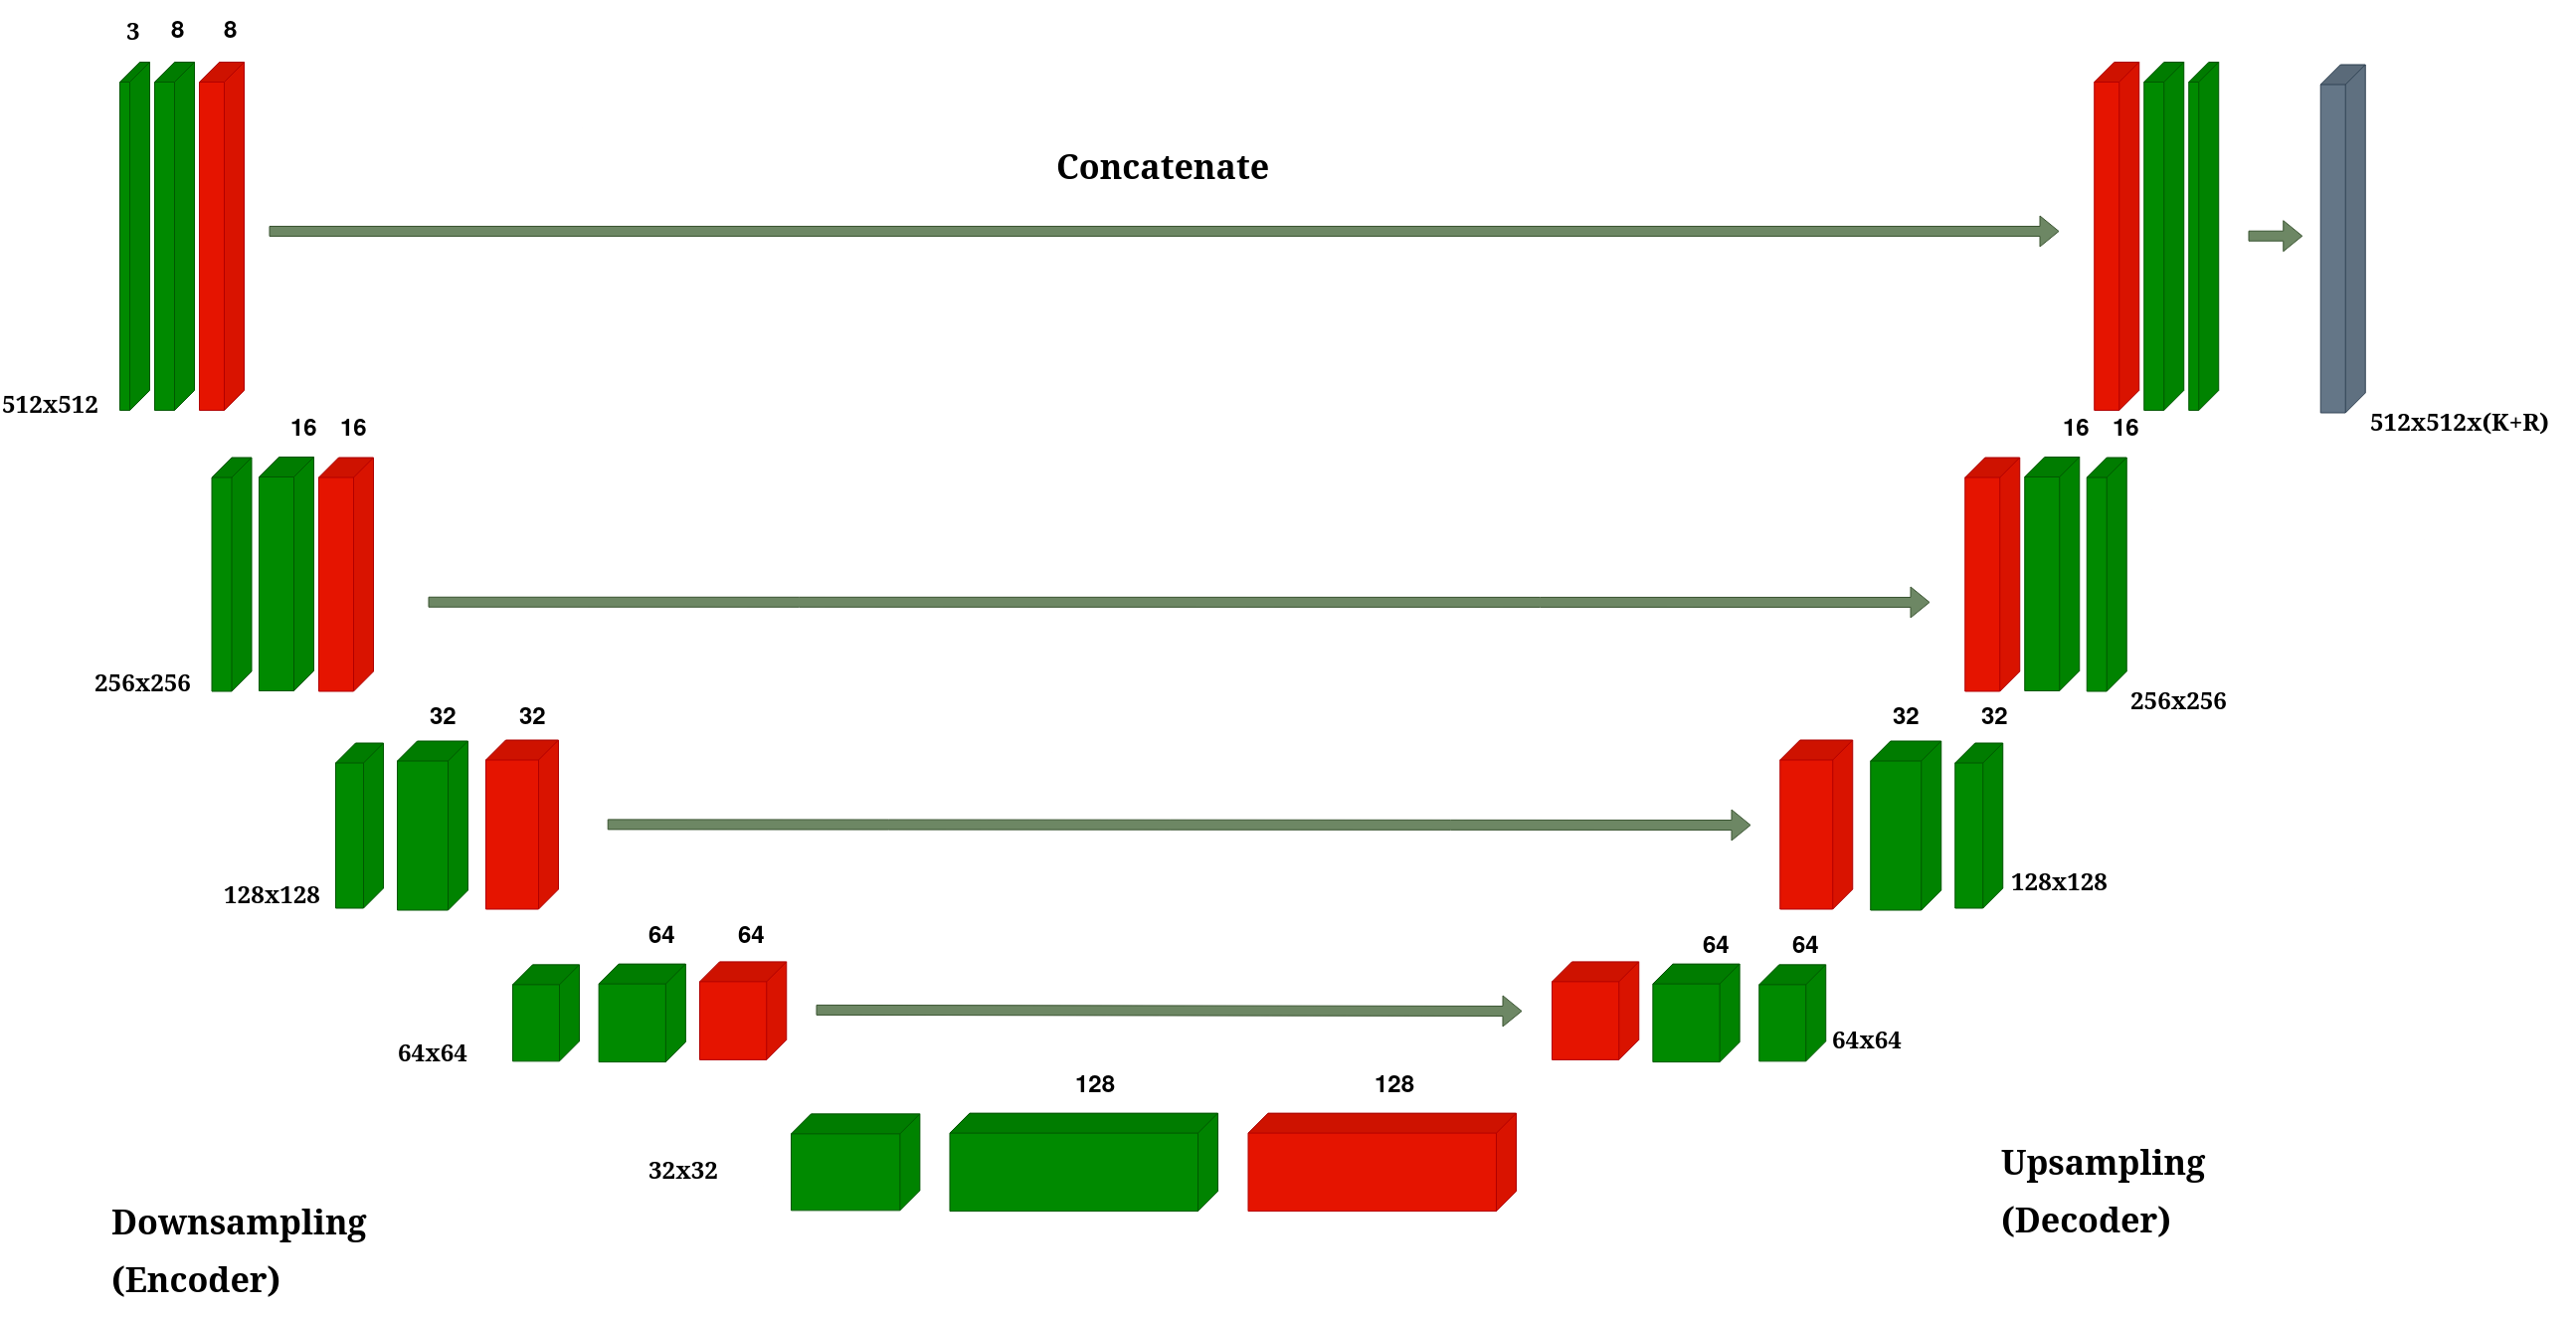
\includegraphics[width=2.5cm]{Cap5/Figures/cnn_arch_overview.png}
    };

    % Output of model
    \node[align=left, right=of image] (modelout) {
      $\left[ f(x; \theta), \; \Lambda_r(x; \theta) \right]$
    };

    % Loss function / objective set
    \node[roundedbox, below=0.7cm of modelout] (loss) {%
      $TGCE_{\text{SS}}(Y_r, f(x;
      \theta) \mid r, \Lambda_r(x; \theta))$
    };

    % Argmin
    \node[box, below=of loss] (argmin) {arg min};

    % Arrows
    \draw[arrow] (dataset) -- (image);
    \draw[arrow] (image) -- (modelout);
    \draw[arrow] (modelout) -- (loss);
    \draw[arrow] (dataset) |- (loss);
    \draw[arrow] (loss) -- (argmin);

  \end{tikzpicture}
  \caption{Training process of the proposed model overview. Estimated
    segmentation and reliability maps are computed for each input
  image, and the loss function is computed for the entire batch.}
  \label{fig:optimization_process}
\end{figure}

The model's architecture is specifically designed to address the
challenges of multi-annotator segmentation. Through the ResNet-34
backbone, it learns robust segmentation features that capture
high-level patterns in the data. The UNET's skip connections enable
the preservation of fine-grained details, while the parallel
reliability branch allows the model to adapt to annotator-specific
characteristics. This comprehensive design enables the model to
effectively handle multiple annotators' inputs while maintaining high
segmentation accuracy and reliability estimation.